%%==================================================
%% abstract.tex for BIT Master Thesis
%% Edited by Jian dahao
%% version: 1.0
%% last update: May 10th, 2019
%%==================================================

\chapter{图表的使用}
\section{插入图片}
\subsection{图片插入基本操作}
\begin{lstlisting}[language={tex}, caption={插入图片示例}]
\begin{figure}
 \centering % 设置为居中显示
 %这里指定图片宽度和图片存放路径
 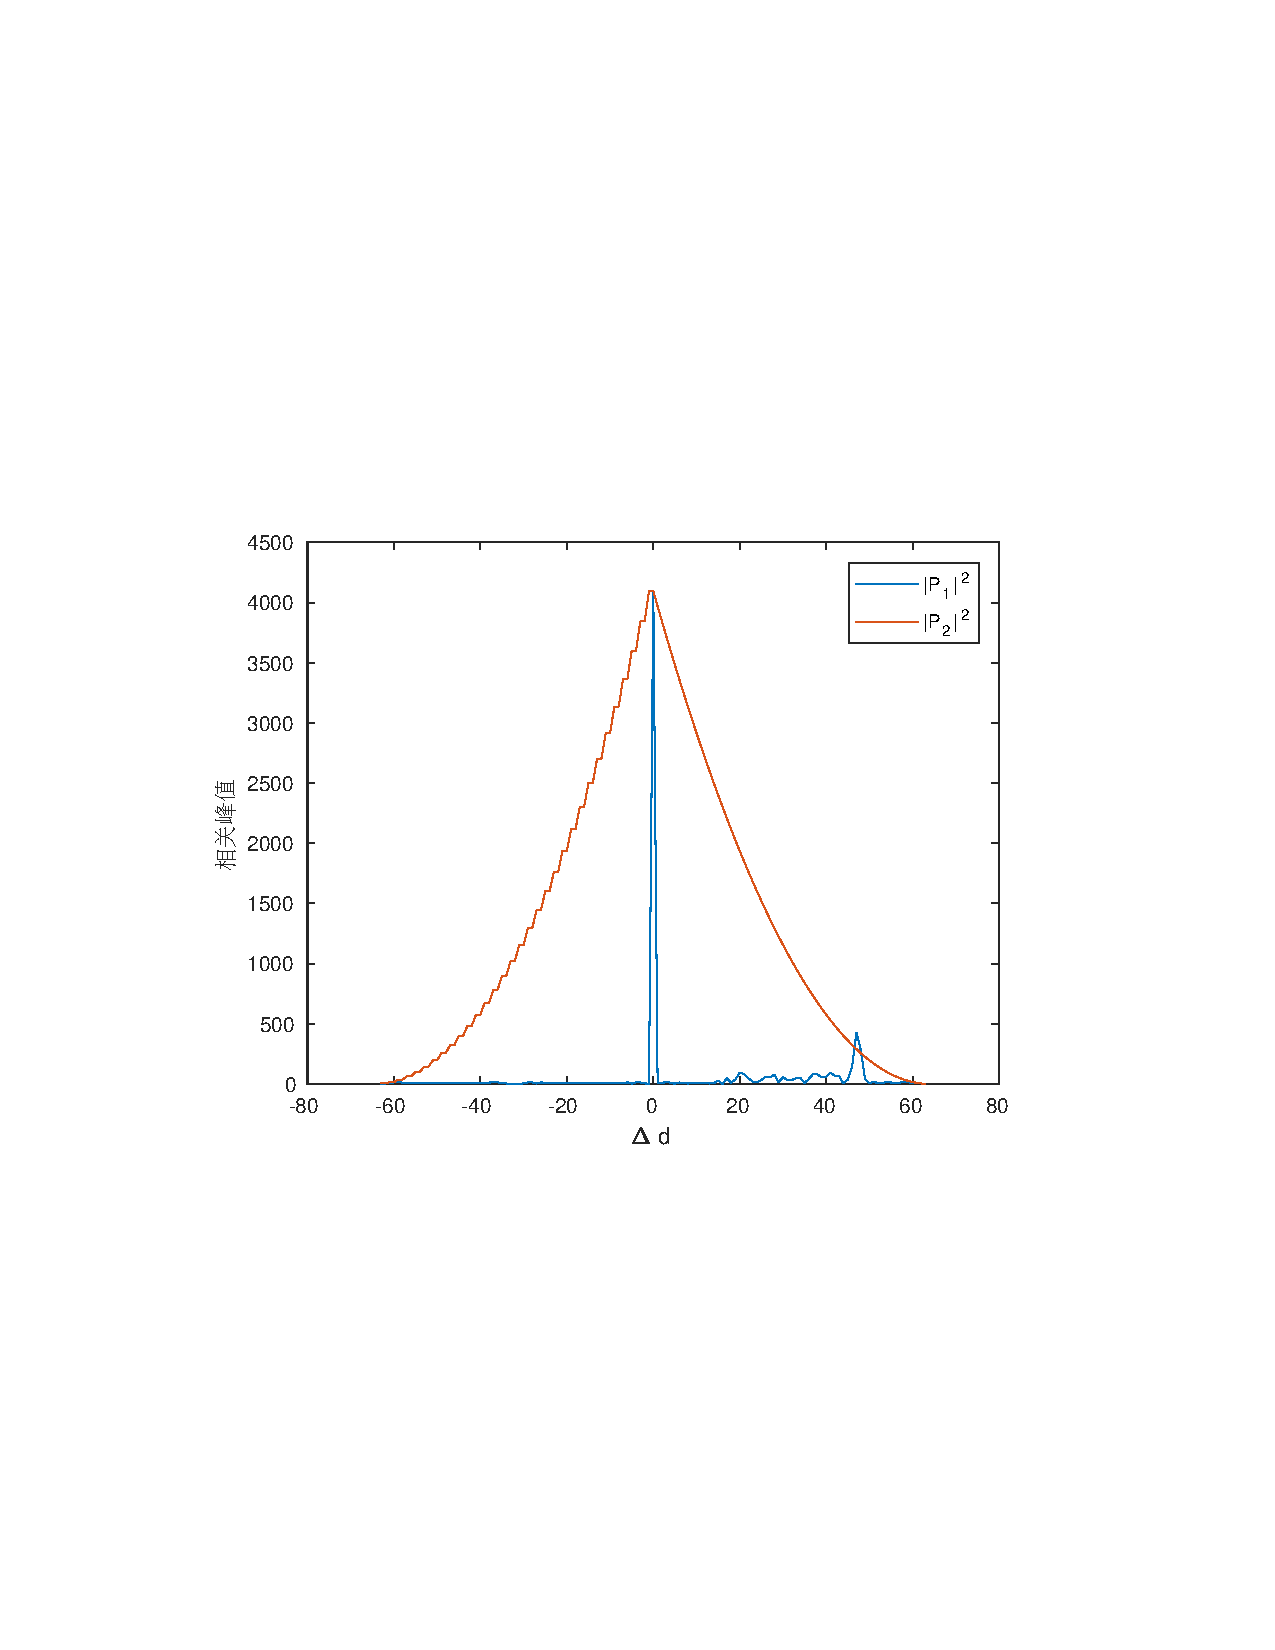
\includegraphics[width=0.75\textwidth]{chapters/figures/correlation_P.pdf}
 \caption{这是标题}%添加图片标题
 \label{fig:figlabel}%设置文件标签,通过$\backslash$ref\{fig:figlabel\}引用
\end{figure}
\end{lstlisting}
\begin{figure}[h]
 \centering
 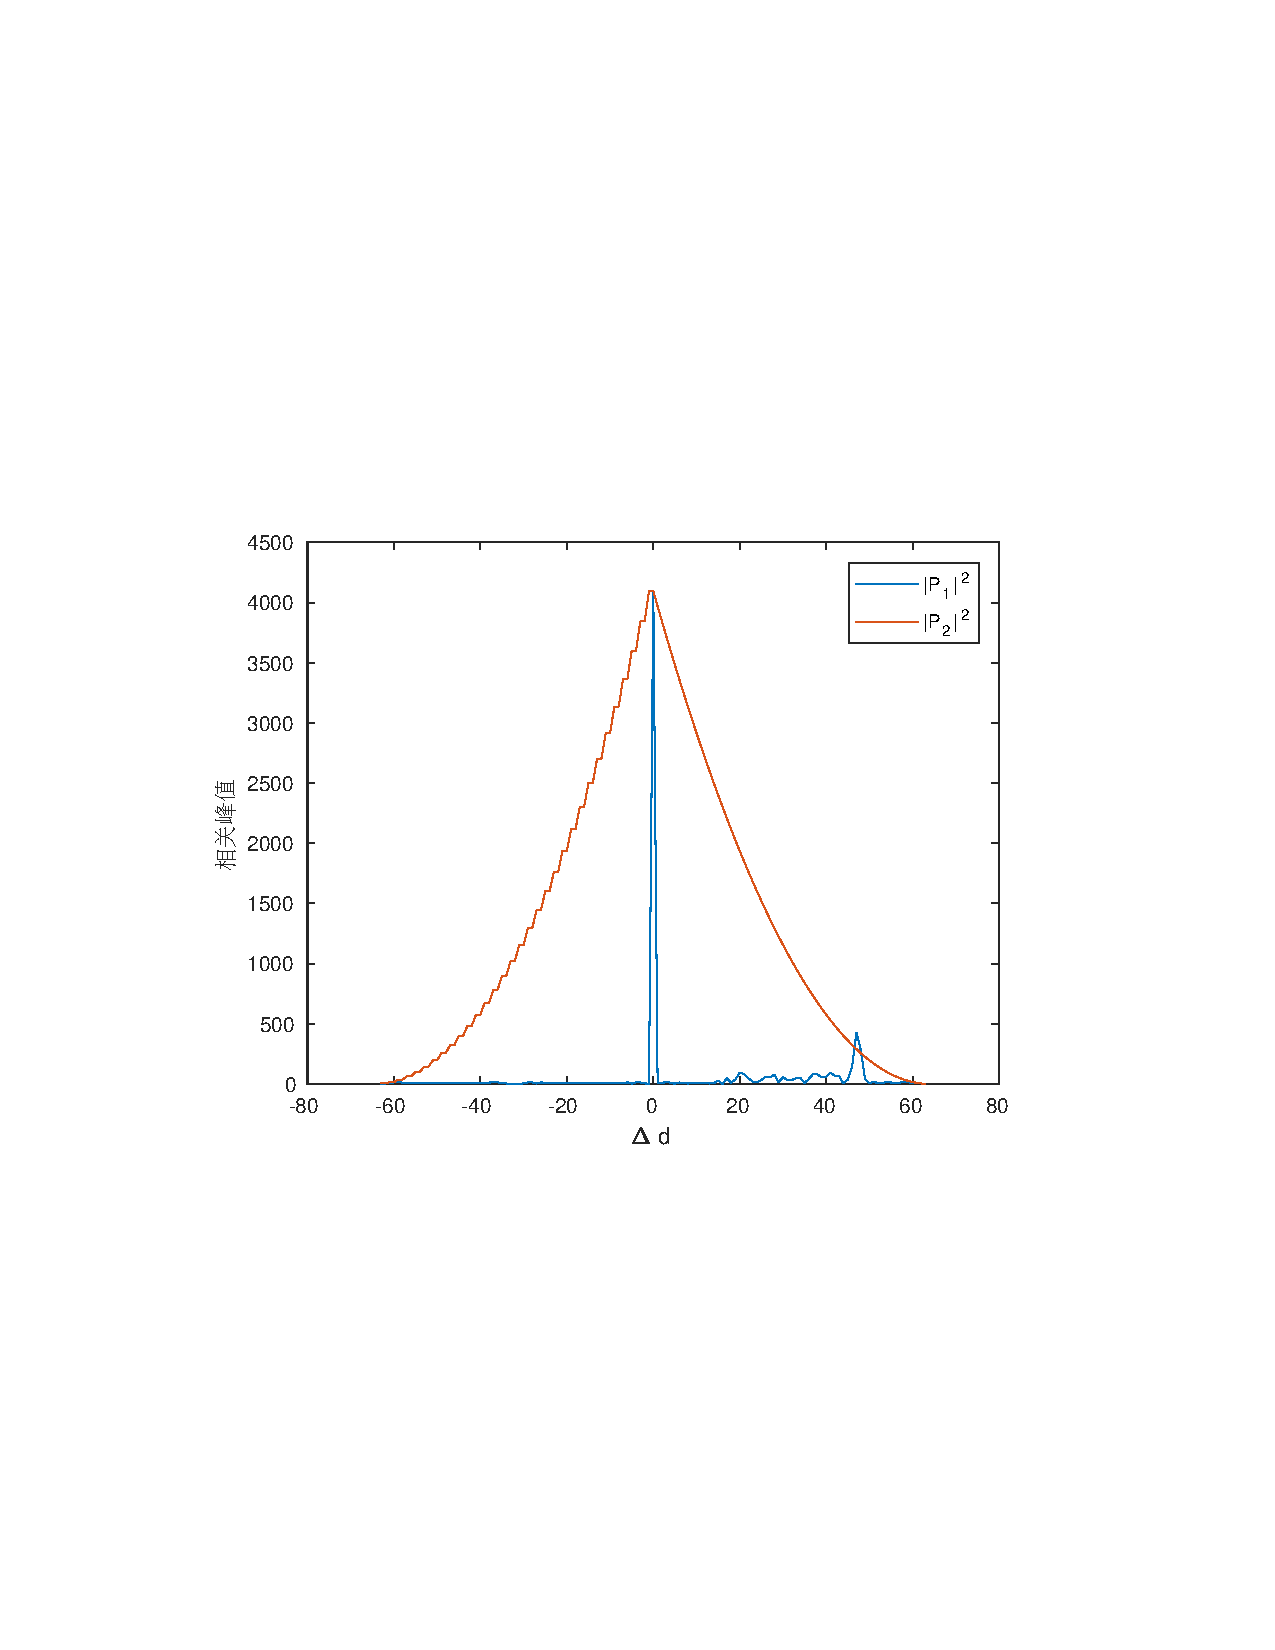
\includegraphics[width=0.75\textwidth]{chapters/figures/correlation_P.pdf}
 \caption{这是标题}\label{fig:correlation_P1_P2}
\end{figure}
\subsection{插入多个子图}
主要通过$\backslash$subfigure完成子图的创建。改变图片的宽度(即width的值)即可实现图片的横排或者竖排效果。

\begin{lstlisting}[language={tex}, caption={插入多个子图示例}]
\begin{figure}
 \centering
 \subfigure[这是第一个子图标题]{
 \label{fig:OFDM_spectrum:a}
 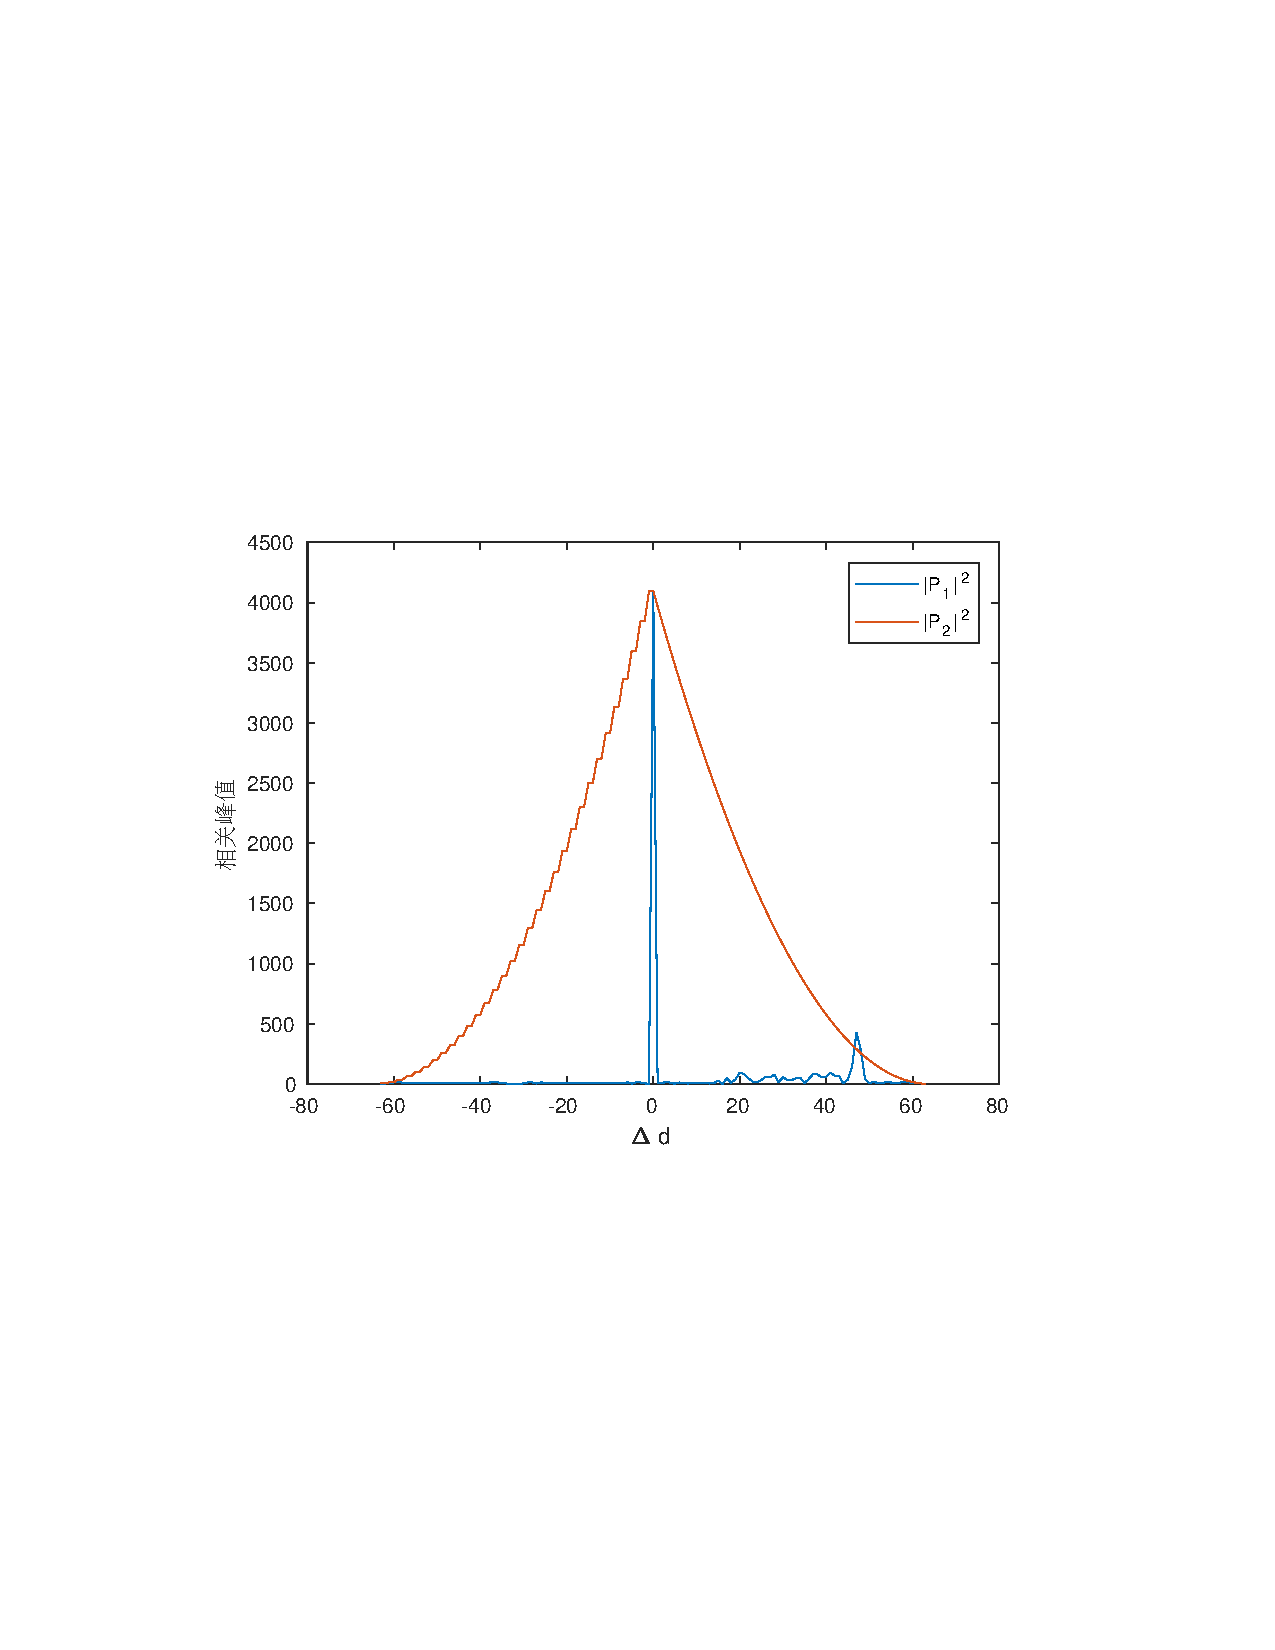
\includegraphics[width=0.48\textwidth]{chapters/figures/correlation_P.pdf}}
 \subfigure[这是第二个子图标题]{
 \label{fig:OFDM_spectrum:b}
 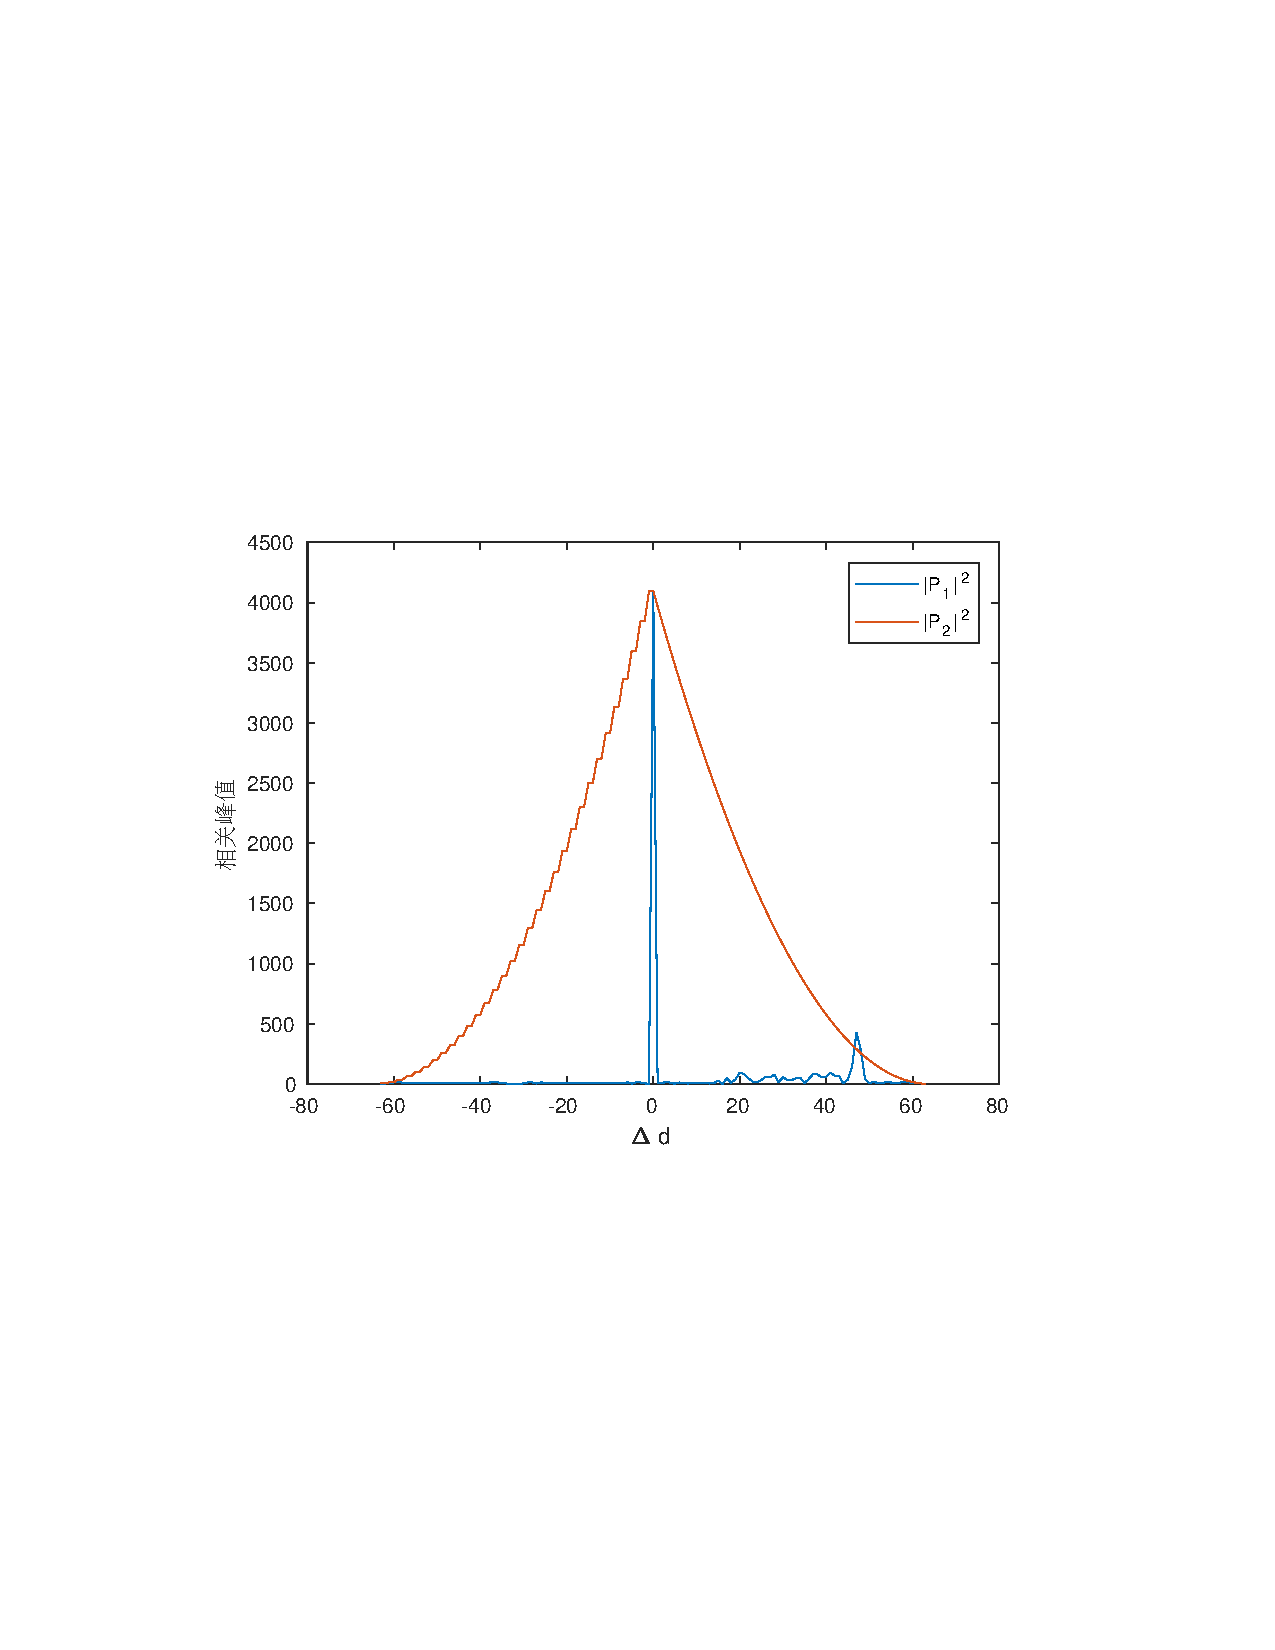
\includegraphics[width=0.48\textwidth]{chapters/figures/correlation_P.pdf}}
 \caption{这是总的图标题}
 \label{fig:OFDM_spectrum}
\end{figure}
\end{lstlisting}
\begin{figure}[h]
 \centering
 \subfigure[这是第一个子图标题]{%创建一个子图
 \label{fig:OFDM_spectrum:a}%设置文件标签,通过$\backslash$ref\{fig:OFDM_spectrum:a\}引用
 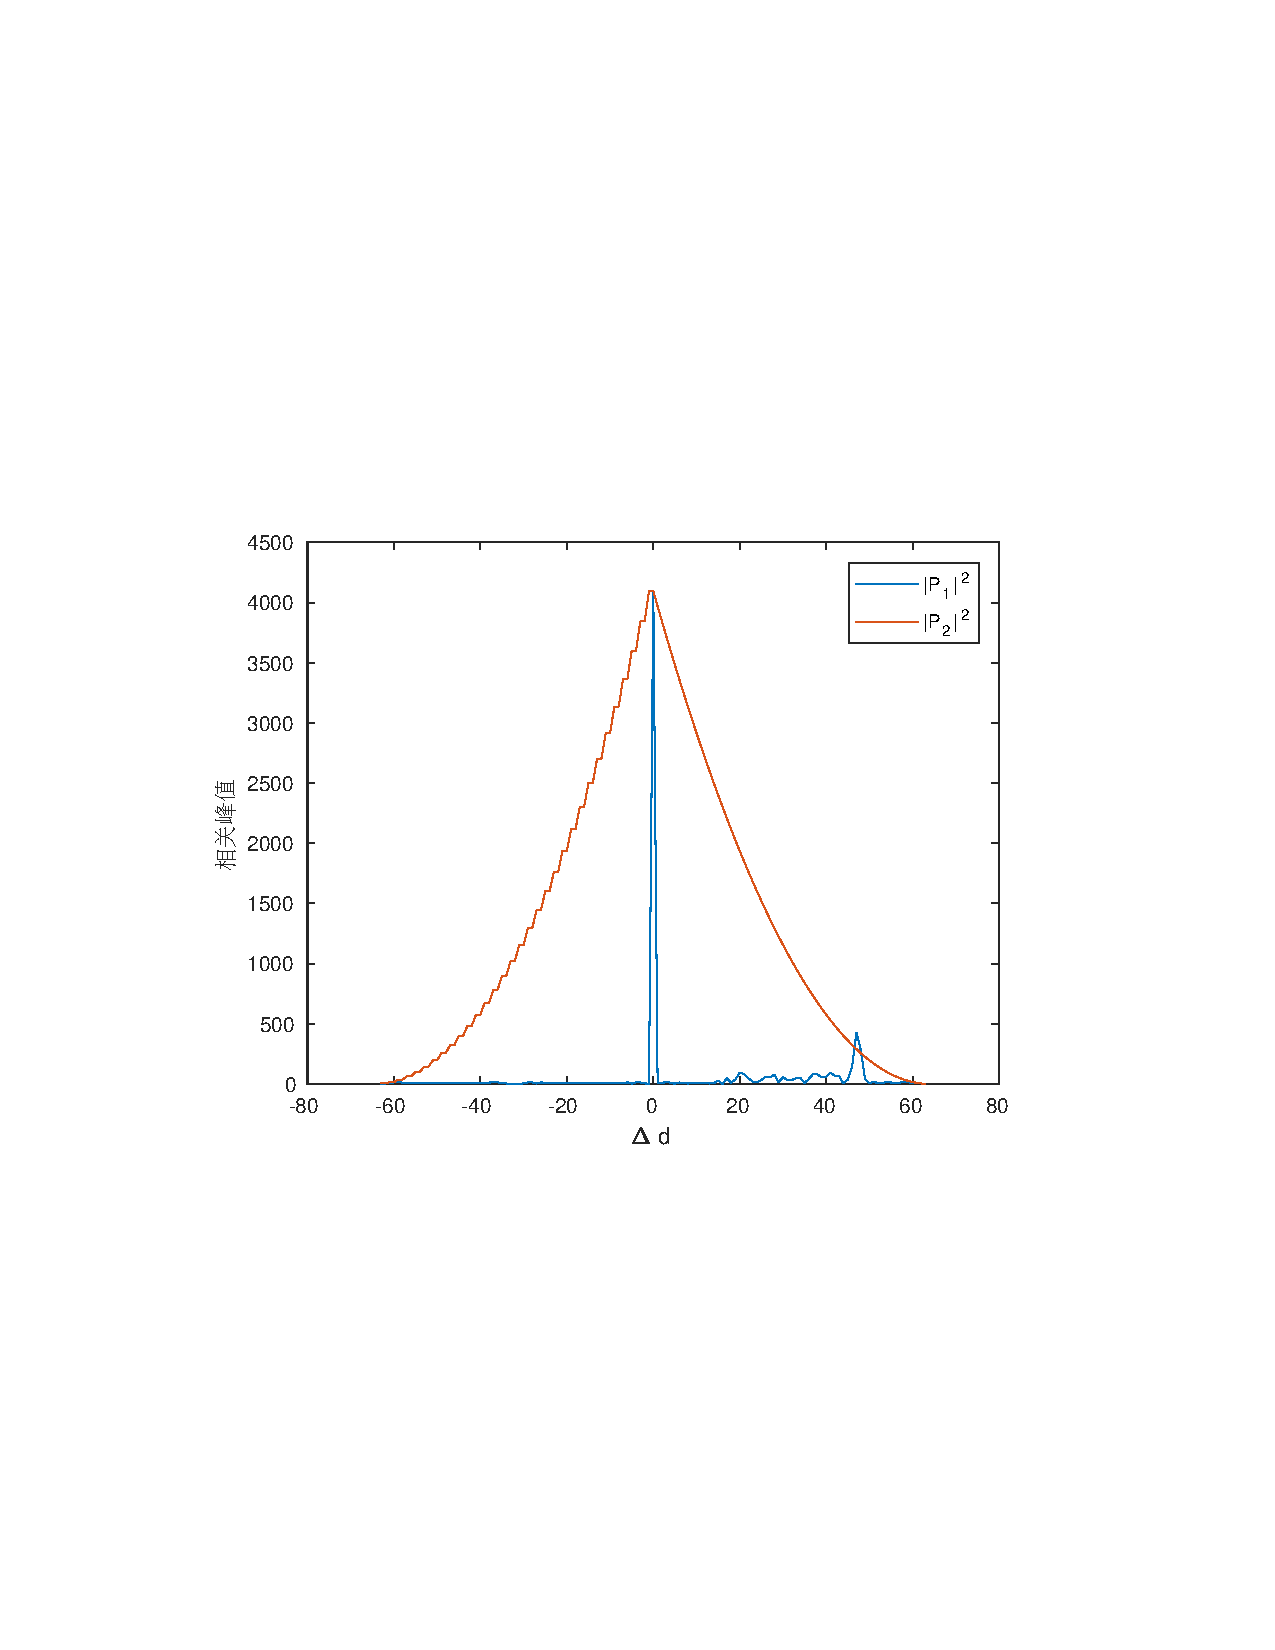
\includegraphics[width=0.48\textwidth]{chapters/figures/correlation_P.pdf}}
 \subfigure[这是第二个子图标题]{
 \label{fig:OFDM_spectrum:b}
 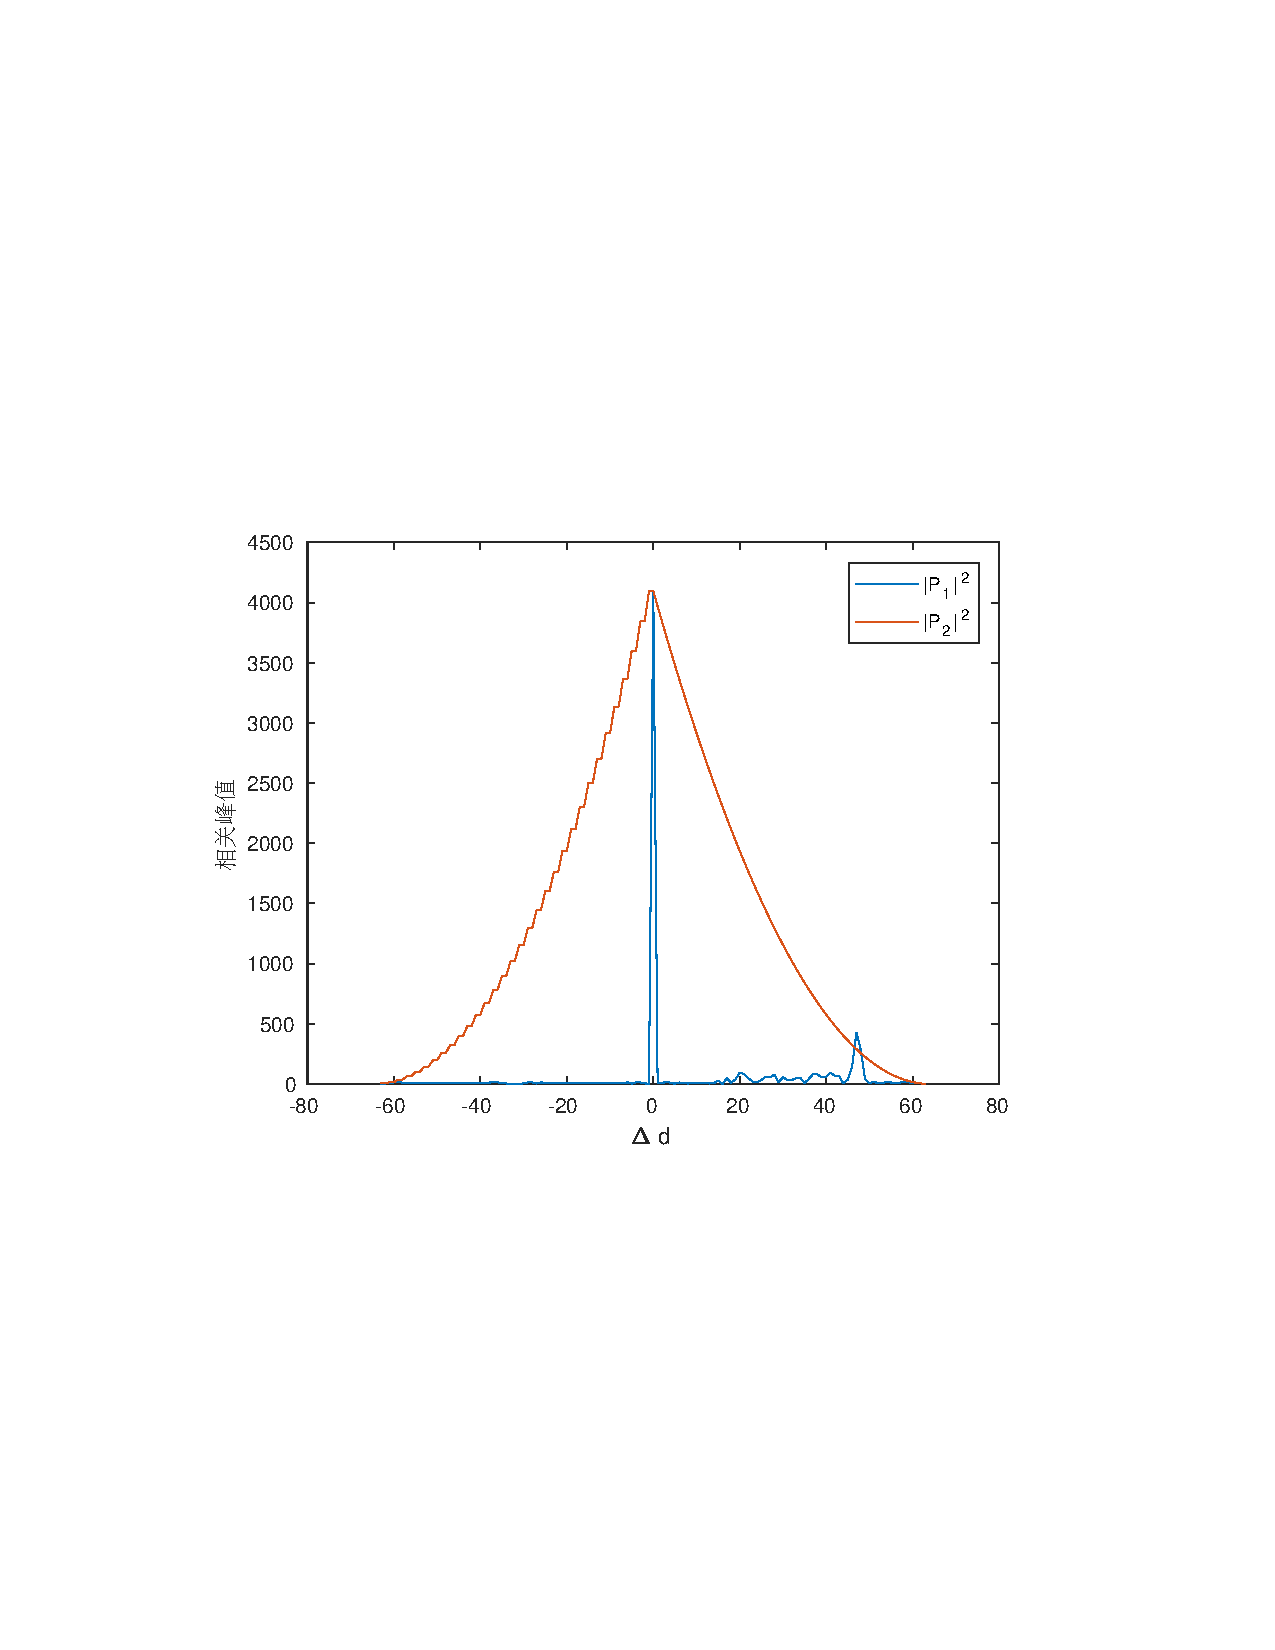
\includegraphics[width=0.48\textwidth]{chapters/figures/correlation_P.pdf}}
 \caption{这是总的图标题}
 \label{fig:OFDM_spectrum}
\end{figure}
\subsection{插图位置乱跑怎么办}
默认情况下图片的位置会被自动安排在合适的地方,当需要自行设置图片位置时可以加入图片浮动格式设置。
\vspace{-0.5cm}
\begin{lstlisting}[language={tex}, caption={设置图片位置示例}]
\begin{figure}[h]%[h] 指定将图片放置在当前位置(文中给出该图形环境的地方
 \centering 
 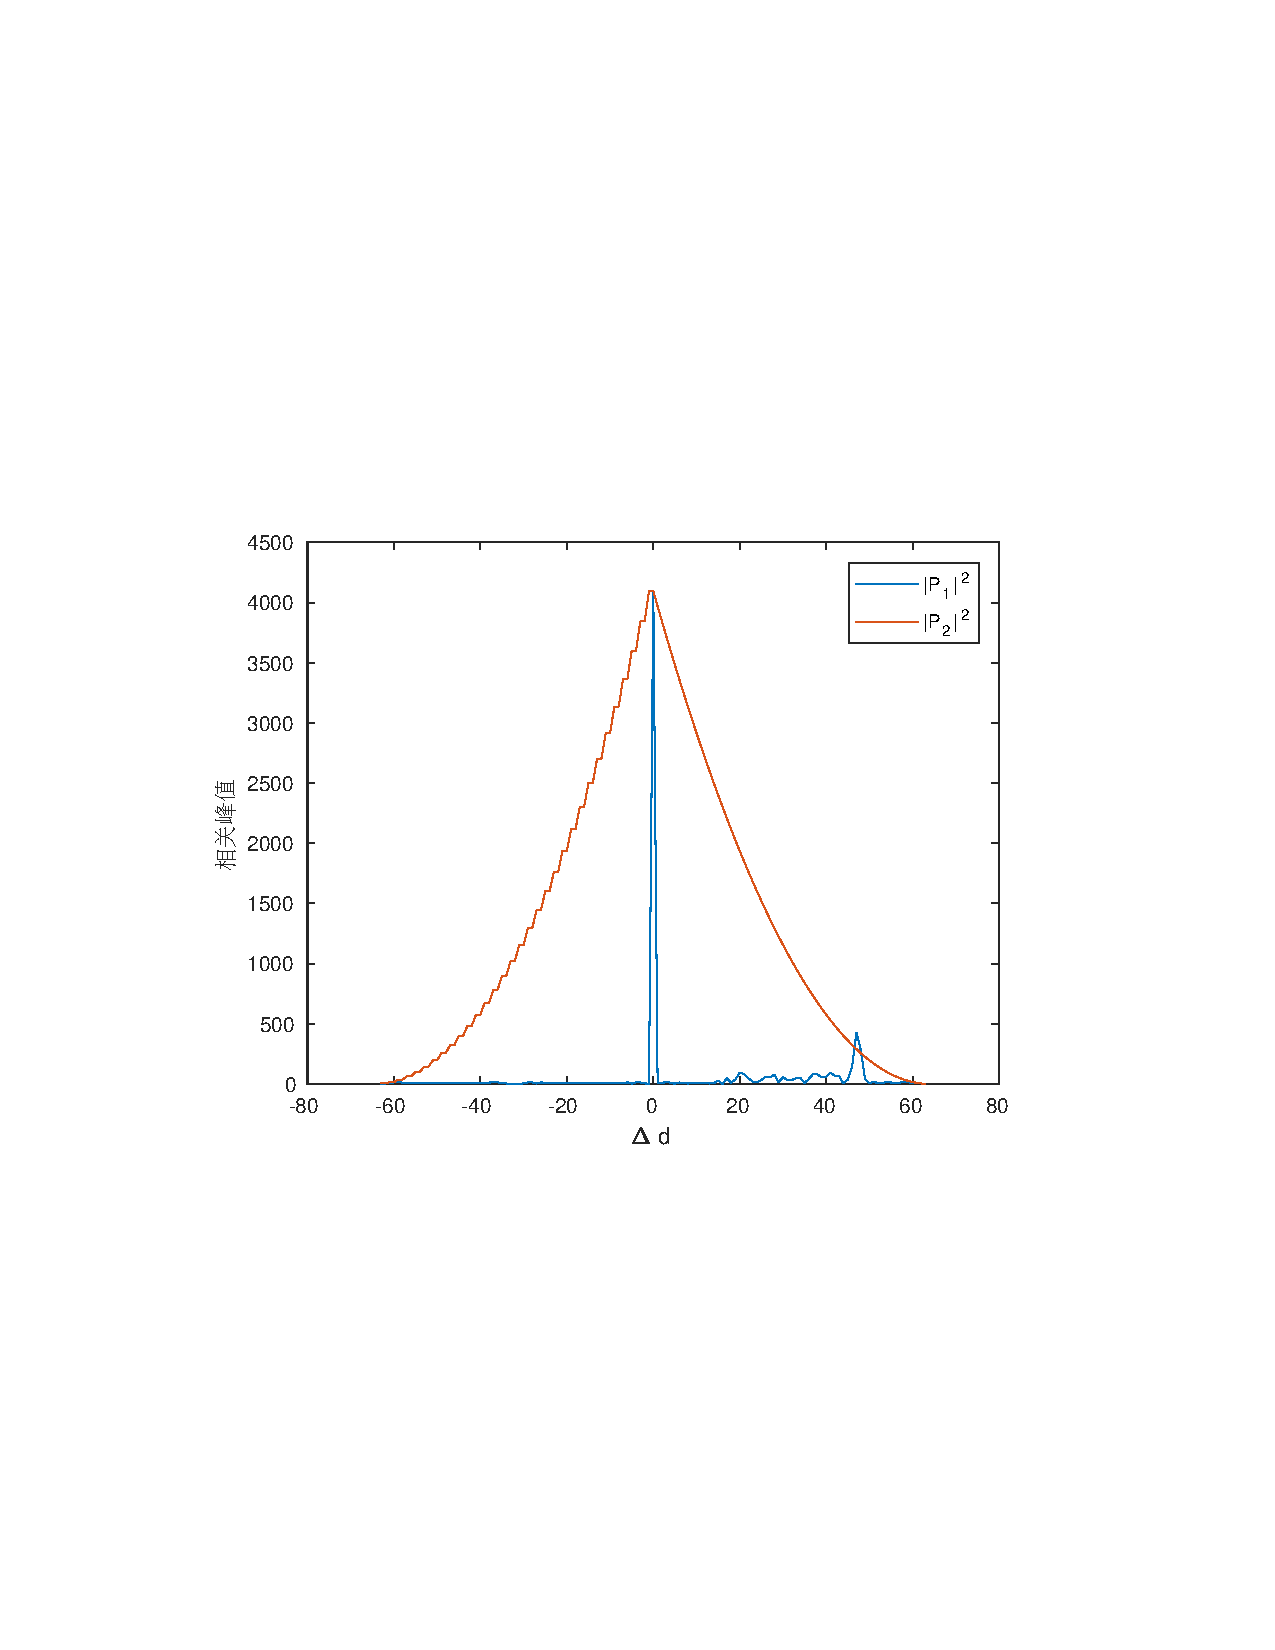
\includegraphics[width=0.75\textwidth]{chapters/figures/correlation_P.pdf}
 \caption{这是标题}
 \label{fig:figlabel}
\end{figure}
\end{lstlisting}
类似的有:

\noindent\fbox{\shortstack[l]{h:当前位置。将图形放置在正文文本中给出该图形环境的地方。如果本页所剩的页面不够,\\ \ \ \ \ 这一参数将不起作用\\
t:将图形放置在页面的顶部。\\
b:将图形放置在页面的底部。\\
p:浮动页。将图形放置在一只允许有浮动对象的页面上。}}

如果加入浮动格式设置后,还是没在预想的位置显示图片怎么办,这通常是由于当前位置剩余的空间偏小,无法放下一张图片。这时可以从以下几个方法去尝试:\\
\noindent{1.改变文本内容和图片定义的位置,给插图腾出足够的显示空间。\\}
\noindent{2.改变段落与图片之间的间距,可以试图使用类似$\backslash$vspace\{-1cm\}这种形式减小间距。\\}
\noindent{3.改变图片的大小,有两种:其一是消除图片多余的白边,其二是减小图片的width值。}

\subsection{插图效果模糊不清晰}
$\XeTeX$可以支持多种图片格式(PDF,EPS,PNG,JPG等),非矢量图片容易造成图片显示不佳,清晰度不高。所以比较推荐使用PDF、EPS等矢量格式,而矢量图中又比较推荐使用PDF格式的图片,因为方便对图片进行编辑和修改(使用Adobe DC可进行编辑)。
\subsection{图片标题太长怎么办}
% \begin{figure}[h]
%  \centering
%  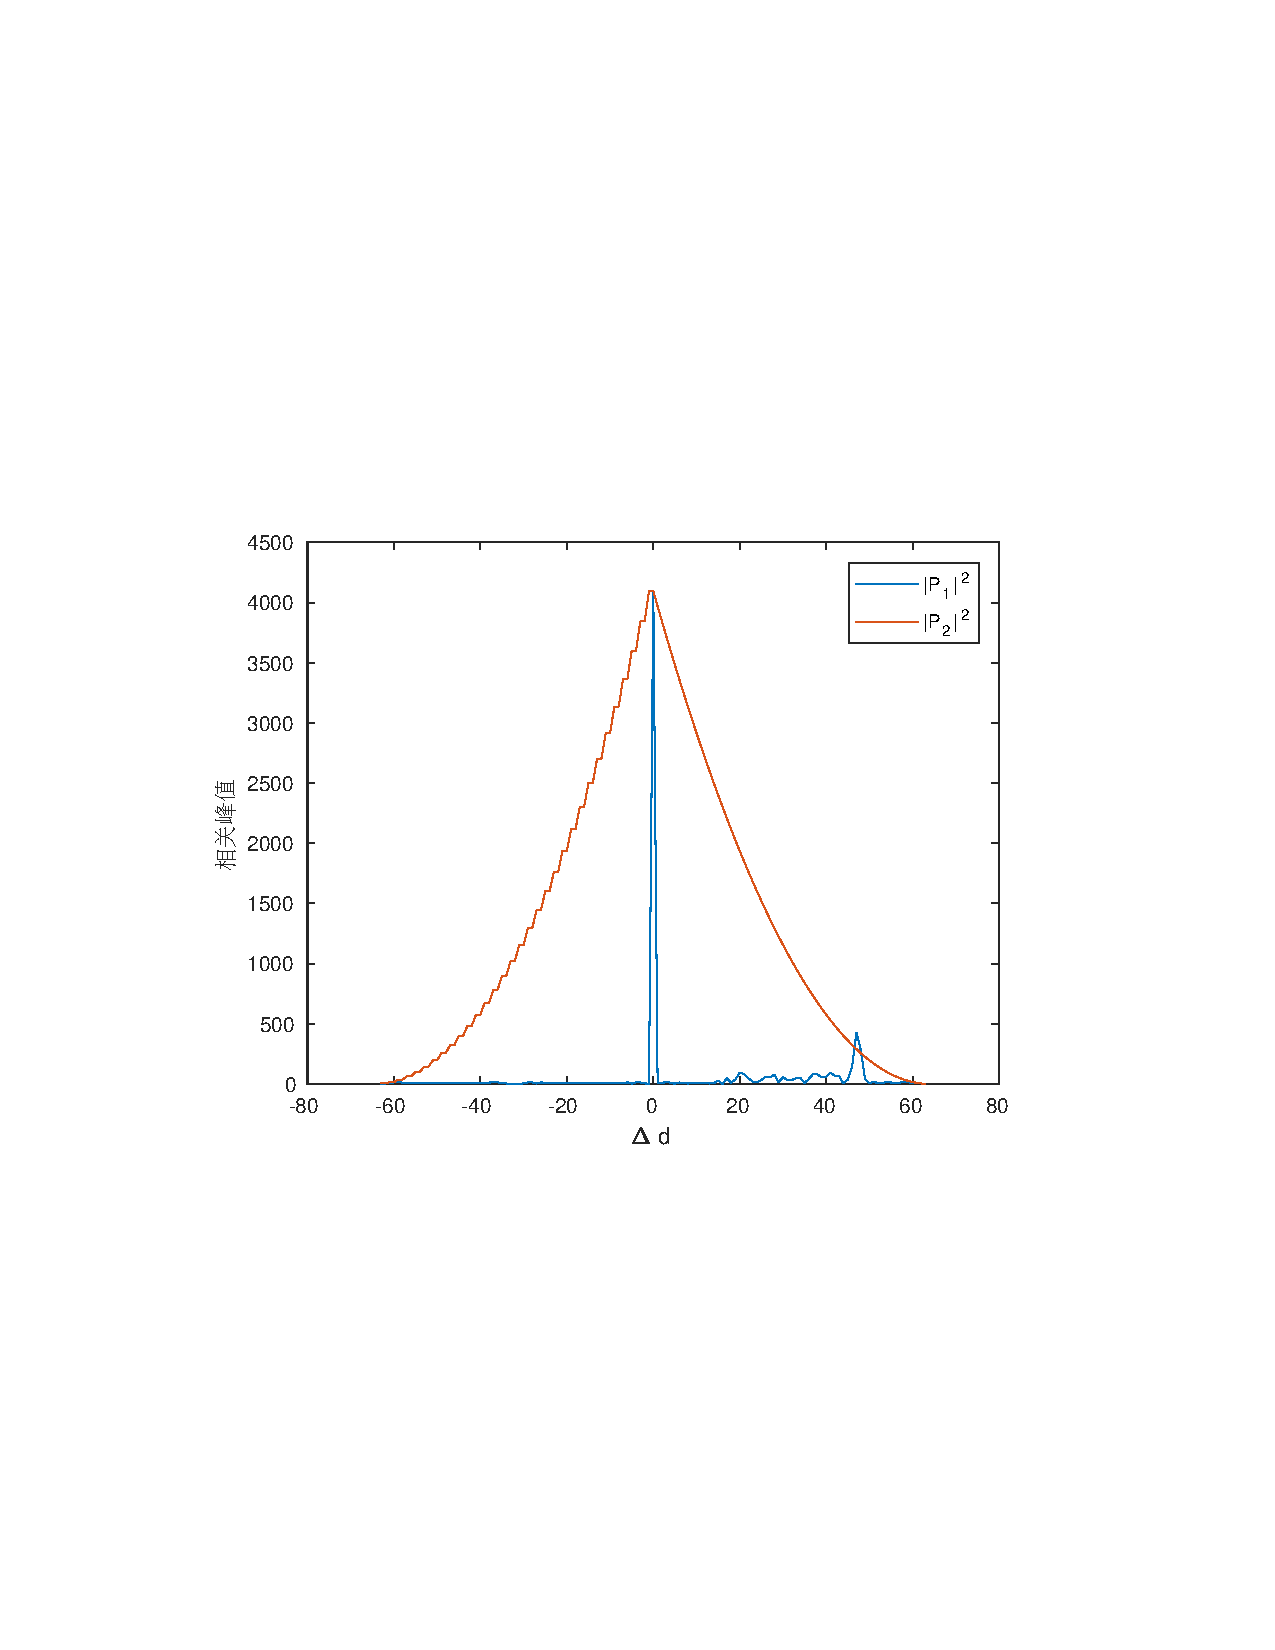
\includegraphics[width=0.75\textwidth]{chapters/figures/correlation_P.pdf}
%  \caption{这是一个很长很长很长很长很长很长很长很长很长很长很长很长很长很长很长很长很长很长很长很长很长的标题}\label{fig:correlation_P1_P2}
% \end{figure}
感觉就是很难看,所以可以想办法让标题在合适的地方自动换行并居中。可以通过添加
\begin{lstlisting}[language={tex}, caption={}]
\usepackage[justification=centering]{caption}
\end{lstlisting}
来实现,这个设置是全局设置。

\subsection{自查重模式下如何关闭图片显示}
在模板BIT-thesis-LaTex中(使用BIT-thesis-grd-jdh.cls格式控制文件)可以使用$\backslash$insertFigure或者$\backslash$insertContents命令来实现。
\begin{lstlisting}[language={tex}, caption={}]
\insertFigure{
	\begin{figure}
		.......
	\end{figure}
}
\insertContents{
	\begin{figure}
		.......
	\end{figure}
}
\end{lstlisting}
% \begin{figure}[h]
%  \centering
%  \label{fig:correlation_P1_P2}
%  % \captionstyle{\centering}
%  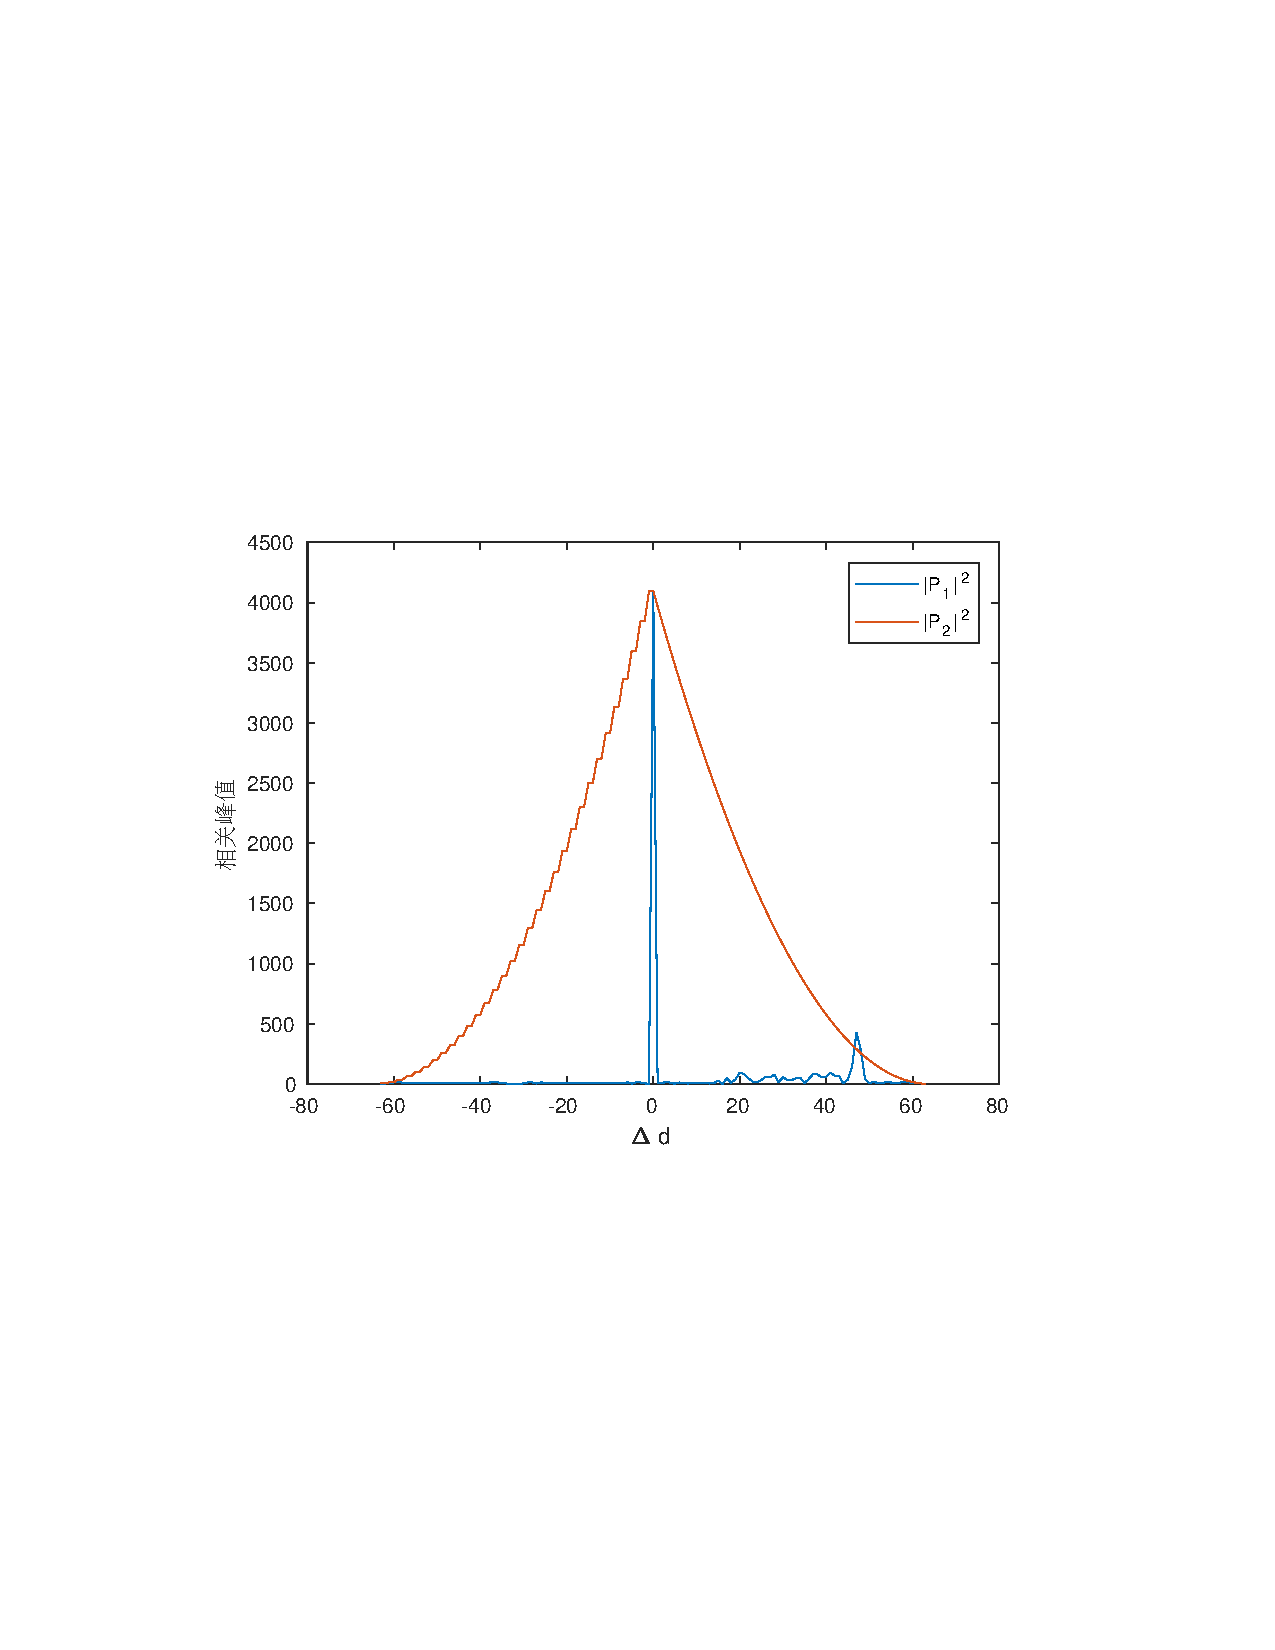
\includegraphics[width=0.75\textwidth]{chapters/figures/correlation_P.pdf}
 
%  \begin{minipage}{0.75\textwidth}
%  \caption{这是一个很长很长很长很长很长很长很长很长很长很长很长很长很长很长很长很长很长很长很长}
%  \end{minipage}
 
% \end{figure}
\section{插入表格}
\subsection{表格制作}
LaTeX中插入的表格对应的代码就如下所示:
\begin{lstlisting}[language={tex}, caption={}]
\begin{table}[]
\centering
\caption{表格标题}
\label{表格引用标签}
\begin{tabular}{@{}ccccccc@{}}
\toprule
算法    & Minn  & Park  & Ren   & Fang  & Shao  & 改进算法\\ \midrule
时间($\mu s$) & 69.57 & 64.36 & 139.39 & 134.94 & 127.45 & 64.86    \\ \bottomrule
\end{tabular}
\end{table}
\end{lstlisting}
对应的效果为:
\begin{table}[h]
\centering
\caption{表格标题}
\label{表格引用标签}
\begin{tabular}{@{}ccccccc@{}}
\toprule
算法    & Minn  & Park  & Ren   & Fang  & Shao  & 改进算法\\ \midrule
时间($\mu s$) & 69.57 & 64.36 & 139.39 & 134.94 & 127.45 & 64.86    \\ \bottomrule
\end{tabular}
\end{table}

手动敲代码是不可能敲代码的,所以我找了一个清爽的表格编辑工具,这边推荐一个在线表格制作网站\url{http://www.tablesgenerator.com/}。
\begin{figure}[h]
 \centering
 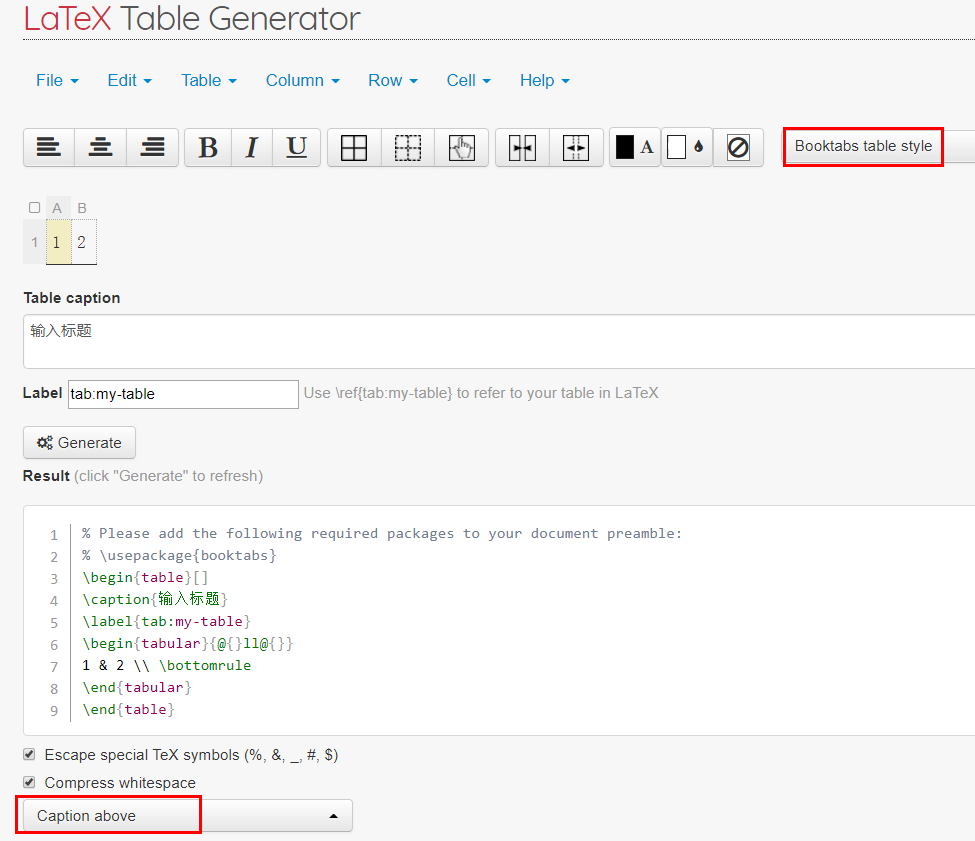
\includegraphics[width=1\textwidth]{chapters/figures/tableGenerator1.png}
 \caption{}
 \label{}
\end{figure}

制作的表格尽量为三线表,编辑好表格后,确保选择为Booktabs table style,然后Generate,复制黏贴就可以了。

\subsection{如何给表格添加脚注}
有时需要给表格添加脚注进行说明,例如:
\begin{table}[h]
\centering
\caption{表格标题}
\begin{threeparttable}
\label{表格引用标签}
\begin{tabular}{@{}ccccccc@{}}
\toprule
算法    & Minn  & Park  & Ren   & Fang  & Shao  & 改进算法\\ \midrule
时间($\mu s$) & 69.57 & 64.36 & 139.39 & 134.94 & 127.45 & 64.86    \\ \bottomrule
\end{tabular}
\begin{tablenotes}
        \footnotesize
        \item[] $N$是OFDM符号长度(不包括循环前缀),也即DFT点数  %此处加入注释信息
        \item[] $\theta$是滑动窗口起始抽样点%此处加入注释信息
      \end{tablenotes}
\end{threeparttable}
\end{table}

对应的代码为:
\begin{lstlisting}[language={tex}, caption={}]
\begin{table}[h] 
\centering
\caption{表格标题}
\begin{threeparttable} % 需要添加的部分
\label{表格引用标签}
\begin{tabular}{@{}ccccccc@{}}
\toprule
算法    & Minn  & Park  & Ren   & Fang  & Shao  & 改进算法\\ \midrule
时间($\mu s$) & 69.57 & 64.36 & 139.39 & 134.94 & 127.45 & 64.86    \\ \bottomrule
\end{tabular}

% 需要添加的部分
\begin{tablenotes}
        \footnotesize
        \item[] $N$是OFDM符号长度(不包括循环前缀),也即DFT点数  %此处加入注释*信息
        \item[] $\theta$是滑动窗口起始抽样点%此处加入注释**信息
      \end{tablenotes}
\end{threeparttable} % 需要添加的部分
\end{table}
\end{lstlisting}
\subsection{自查重模式下如何关闭表格显示}
在模板BIT-thesis-LaTex中(使用BIT-thesis-grd-jdh.cls格式控制文件)可以使用$\backslash$insertTable或者$\backslash$insertContents命令来实现。
\begin{lstlisting}[language={tex}, caption={}]
\insertTable{
	\begin{table}
		.......
	\end{table}
}
\insertContents{
	\begin{table}
		.......
	\end{table}
}
\end{lstlisting}